%% Modified in 2022 by Daniel Bohuněk
%% Created in 2018 by Martin Slapak
%% Based on file for NRP report LaTeX class by Vit Zyka (2008)
\documentclass[english]{mvi-report}

\usepackage[utf8]{inputenc}
\usepackage{amsmath,amssymb,amsthm}
\usepackage{subfig}
\usepackage[colorlinks=true,
            urlcolor=cyan,
            linkcolor=magenta,
            citecolor=magenta]{hyperref}
\usepackage{url}
\def\UrlBreaks{\do\/\do-}

\title{Tire tread superresolution}

\author{Daniel Bohuněk}
\affiliation{Czech Technical University - Faculty of Information Technology}
\email{bohundan@fit.cvut.cz}

\begin{document}

\maketitle

\section{Introduction}
This work expands upon the author's bachelor thesis \cite{Bohunek2022}, in which a camera system for scanning tire treads was devised. This work aims to create a model capable of upscaling tire tread images to improve their sharpness. The model should also compensate for bad focus of the camera when scanning treads from greater distances than anticipated (the camera system is designed to scan just one closest tire but is capable of segmenting other tires present in the scene).

\begin{figure}[htpb]
  \centering
  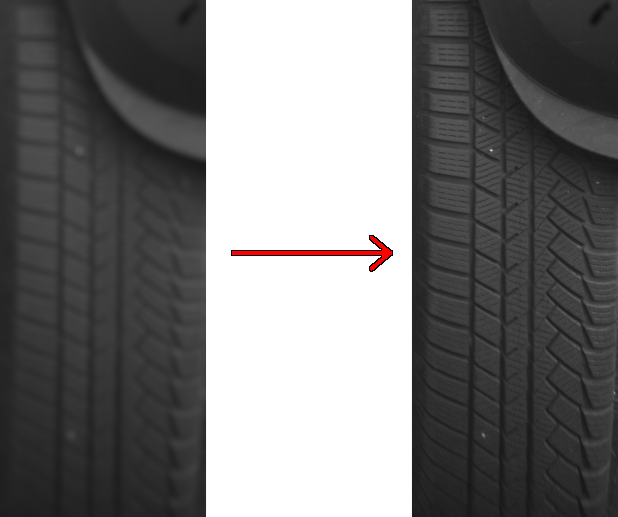
\includegraphics[width=0.8\linewidth]{media/deblurring.png}
  \caption{Goal of this work.}
  \label{fig:deblurring}
\end{figure}

\section{Training data}
315 grayscale images of tire treads were created during the development and testing of the camera system. Postprocessing methods (gradient removal, histogram equalization) were implemented during the student summer research program (VýLet 2022). The equalized images can act as additional augmented data, but this might not be necessary, as the chosen model can learn to upscale accurately with less than a hundred images.

Of the 315 images, 59 high-resolution images were chosen as the training images. Nine other good-quality images plus five low-resolution images act as the testing data so that the model's accuracy can be measured.

\section{Methods}
SRCNN \cite{Dong2014} model was chosen for its simplicity. It processes $64\times64$ subimages, so an image has to be split into so-called \textit{patches} before being fed through the network.

\begin{figure}[htpb]
  \centering
  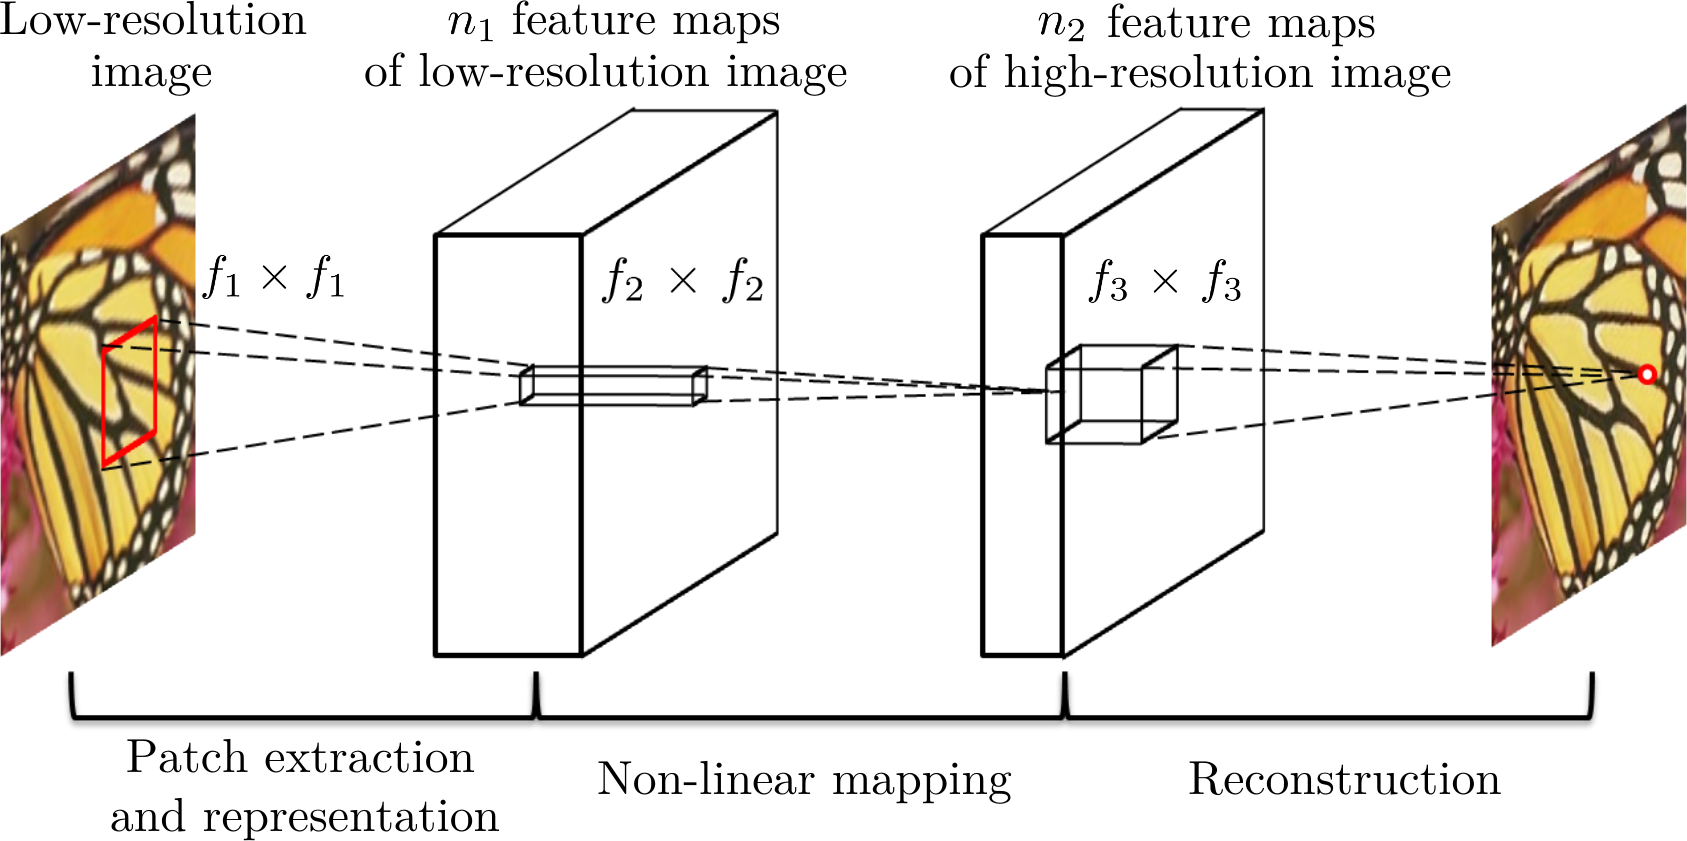
\includegraphics[width=\linewidth]{media/SRCNN-structure.png}
  \caption{SRCNN pipeline \cite{Dong2014}.}
  \label{fig:srcnn-structure}
\end{figure}

Because the tire tread scanning camera system works with grayscale images, the SRCNN model can process just one channel instead of three color channels. To measure the reconstruction accuracy, the peak signal-to-noise ratio (PSNR) can be used:
\begin{equation*}
  \text{PSNR}(I_1, I_2) = 20 \cdot \log_{10} \left( \frac{\text{MAX}_I}{\sqrt{\text{MSE}(I_1, I_2)}} \right),
\end{equation*}
where $I_1$ and $I_2$ are images, $\text{MAX}_I$ is the maximum possible pixel value (usually 255), and $\text{MSE}(I_1, I_2)$ is the mean square error of the two images.

\section{Results}

Splitting each training image into $64\times64$ patches with the stride of $4$ yields a total of 9120 training patches. One training epoch on an RTX 3060 Mobile takes roughly 130 seconds to finish. The authors of the original paper trained their model with ${8\cdot10^8}$ backpropagations. Unfortunately, these many backpropagations are not doable with the available hardware. However, as the original authors noted, many backpropagations are not necessary to achieve good results.

\begin{figure*}[htpb]
    \centerline{
    \subfloat[Original]{
        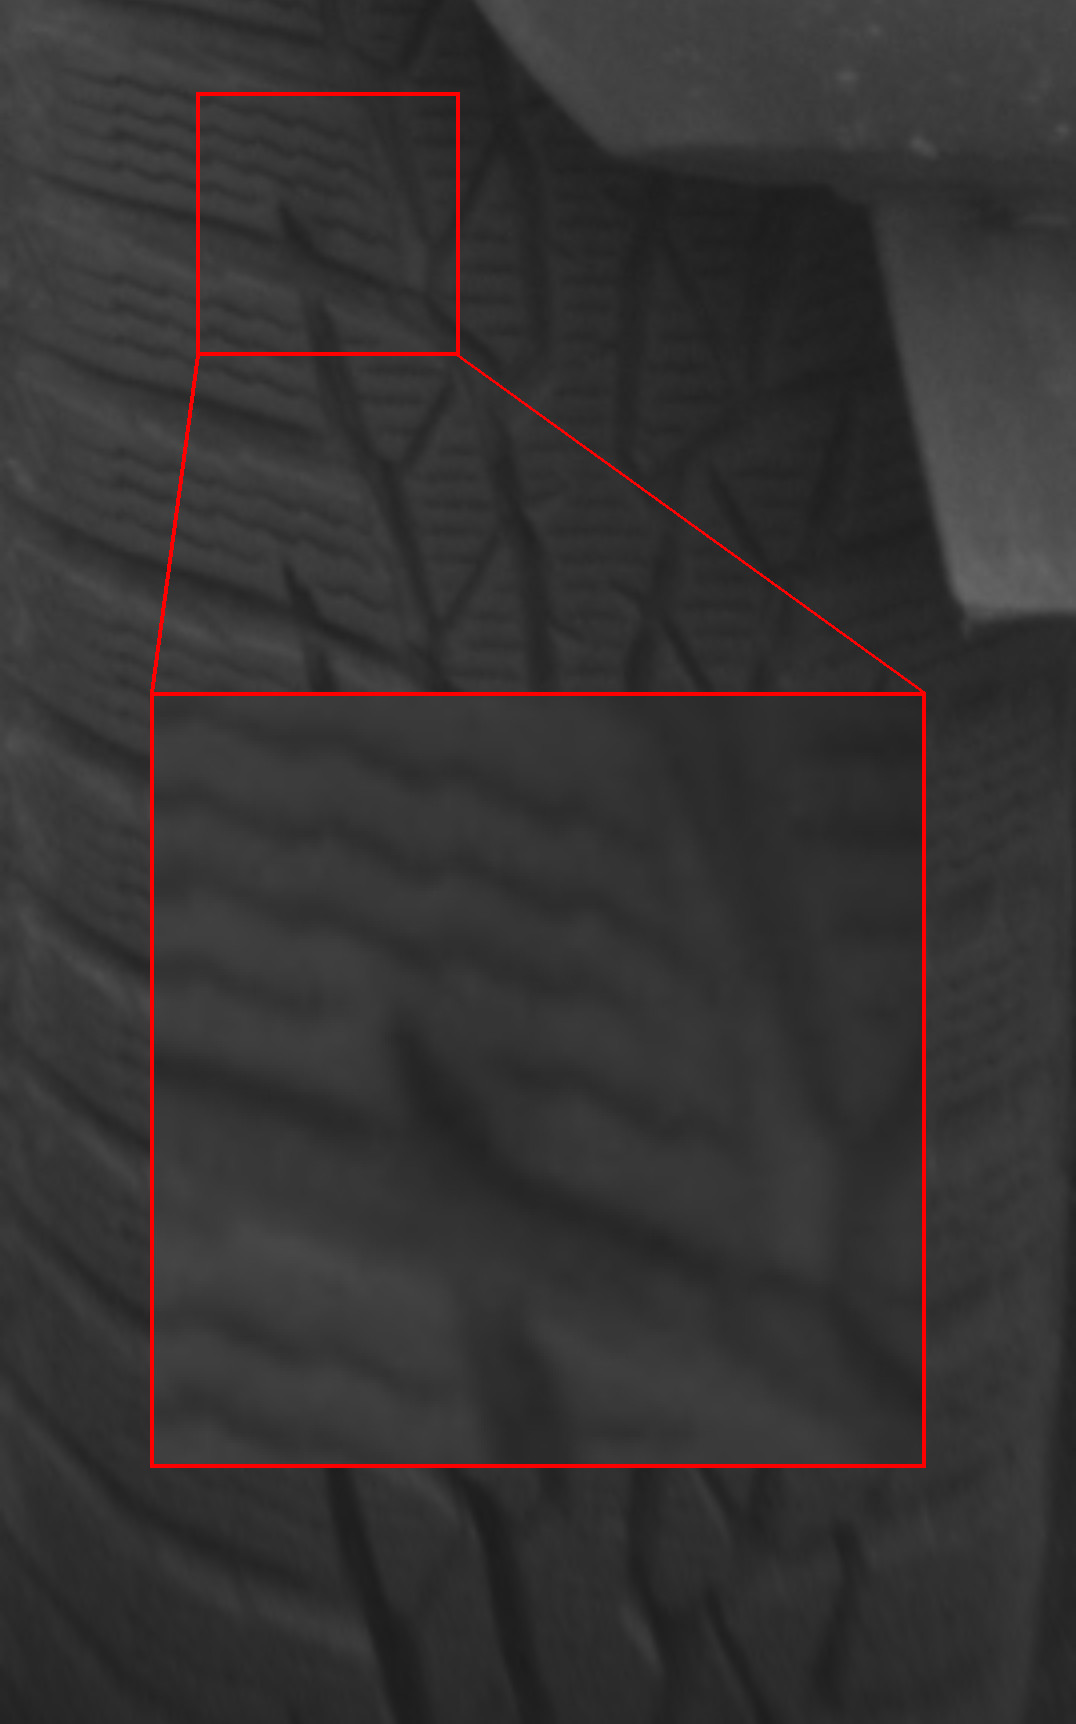
\includegraphics[width=0.2\textwidth]{media/upscaled-original.jpg}
        \label{fig:upscaled-original}
    }
    \subfloat[10 epochs]{
        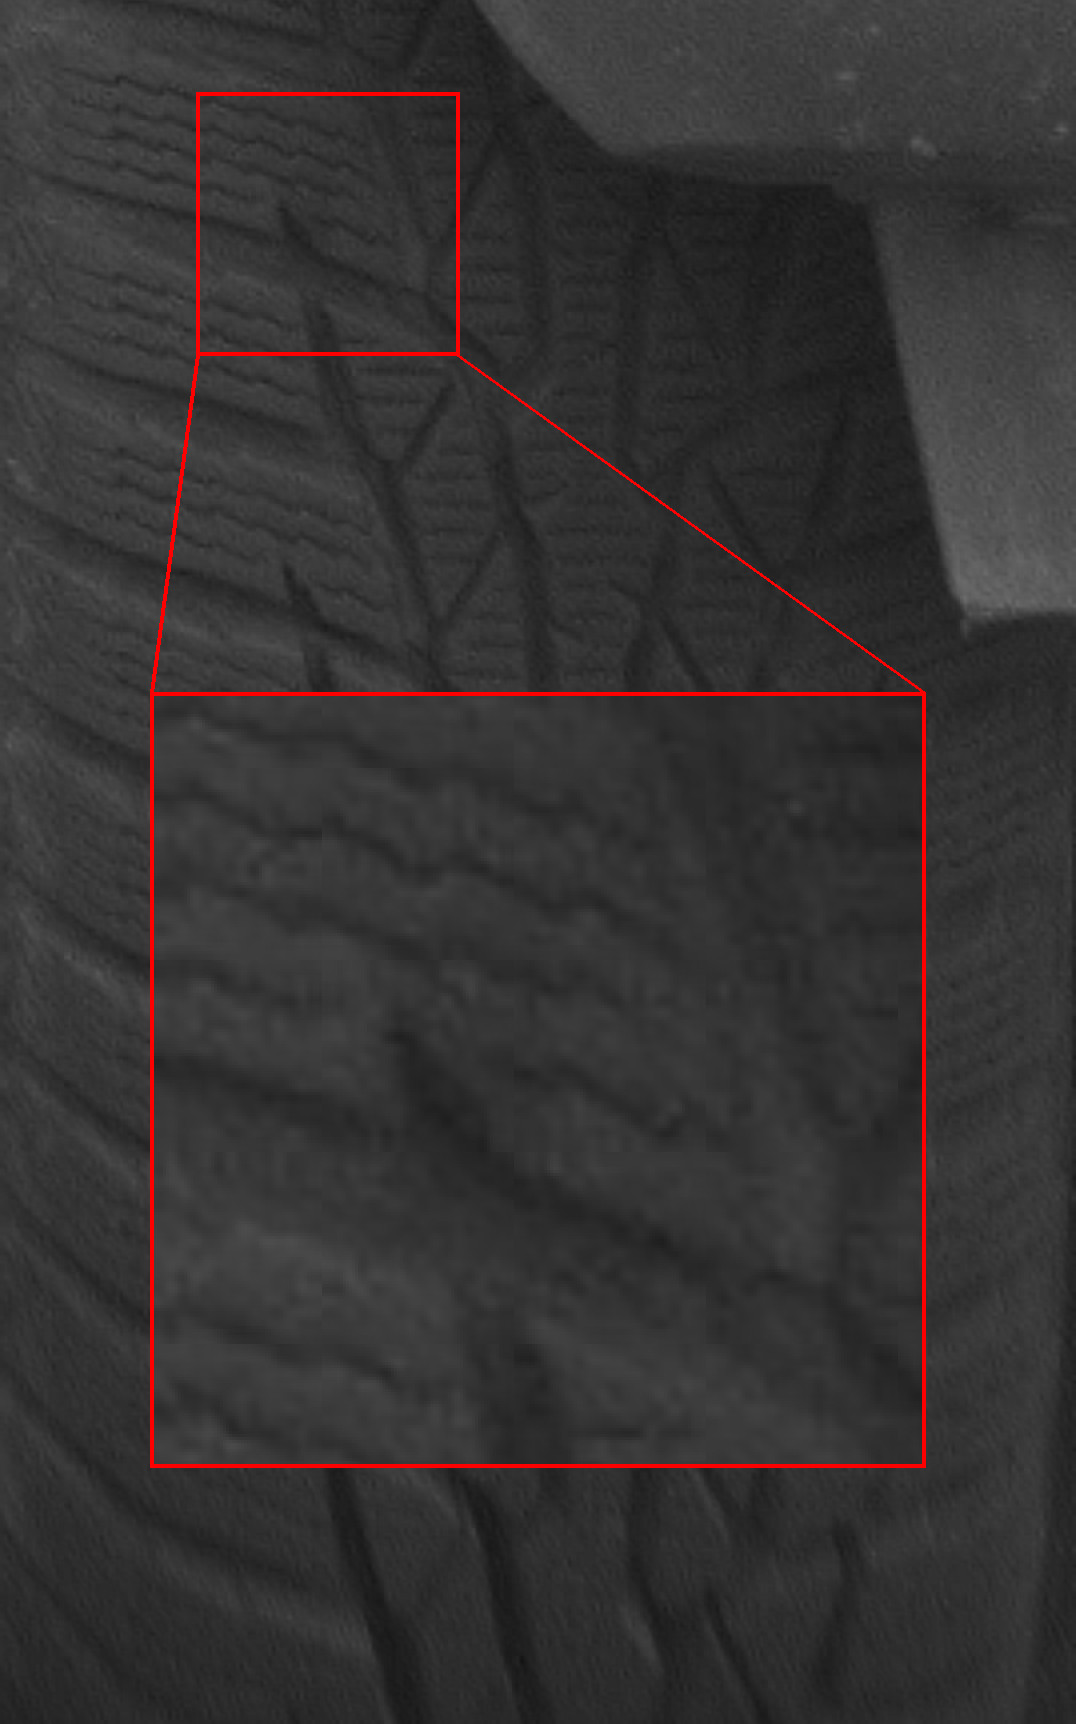
\includegraphics[width=0.2\textwidth]{media/upscaled-10epochs.jpg}
        \label{fig:upscaled-10epochs}
    }
    \subfloat[250 epochs]{
        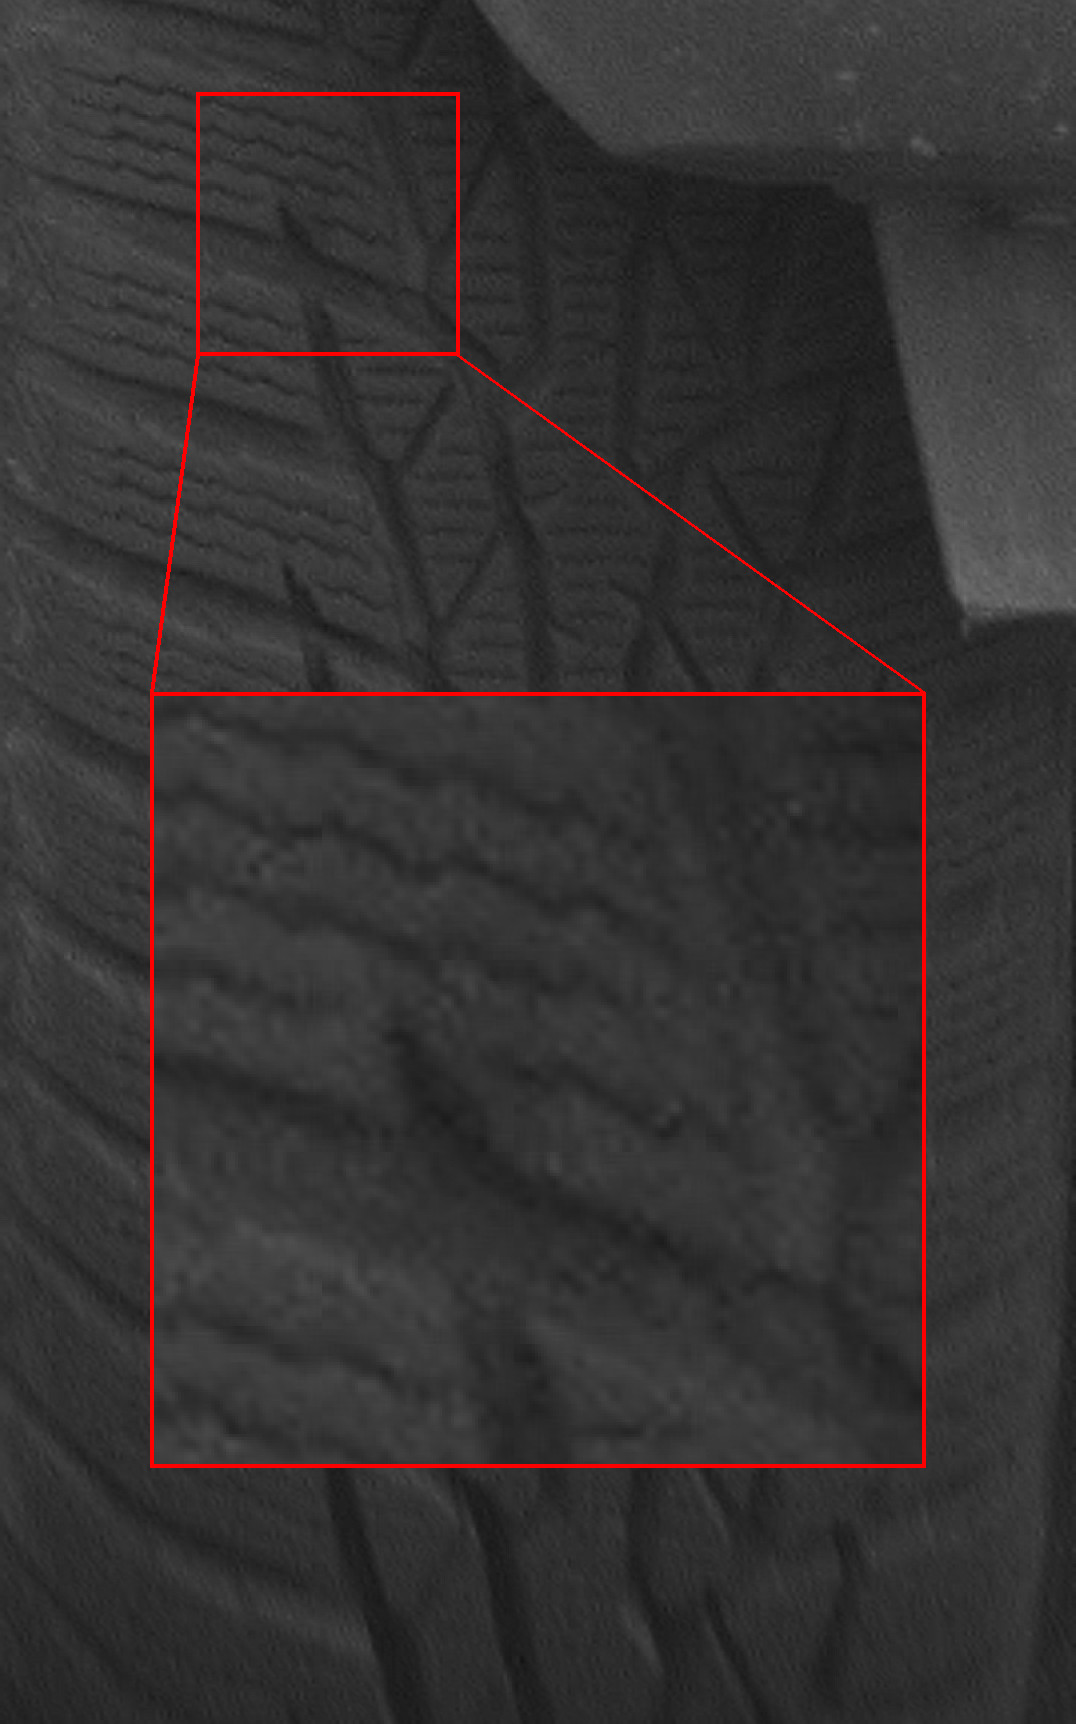
\includegraphics[width=0.2\textwidth]{media/upscaled-250epochs.jpg}
        \label{fig:upscaled-250epochs}
    }
    \subfloat[250 epochs with \break less downsampling]{
        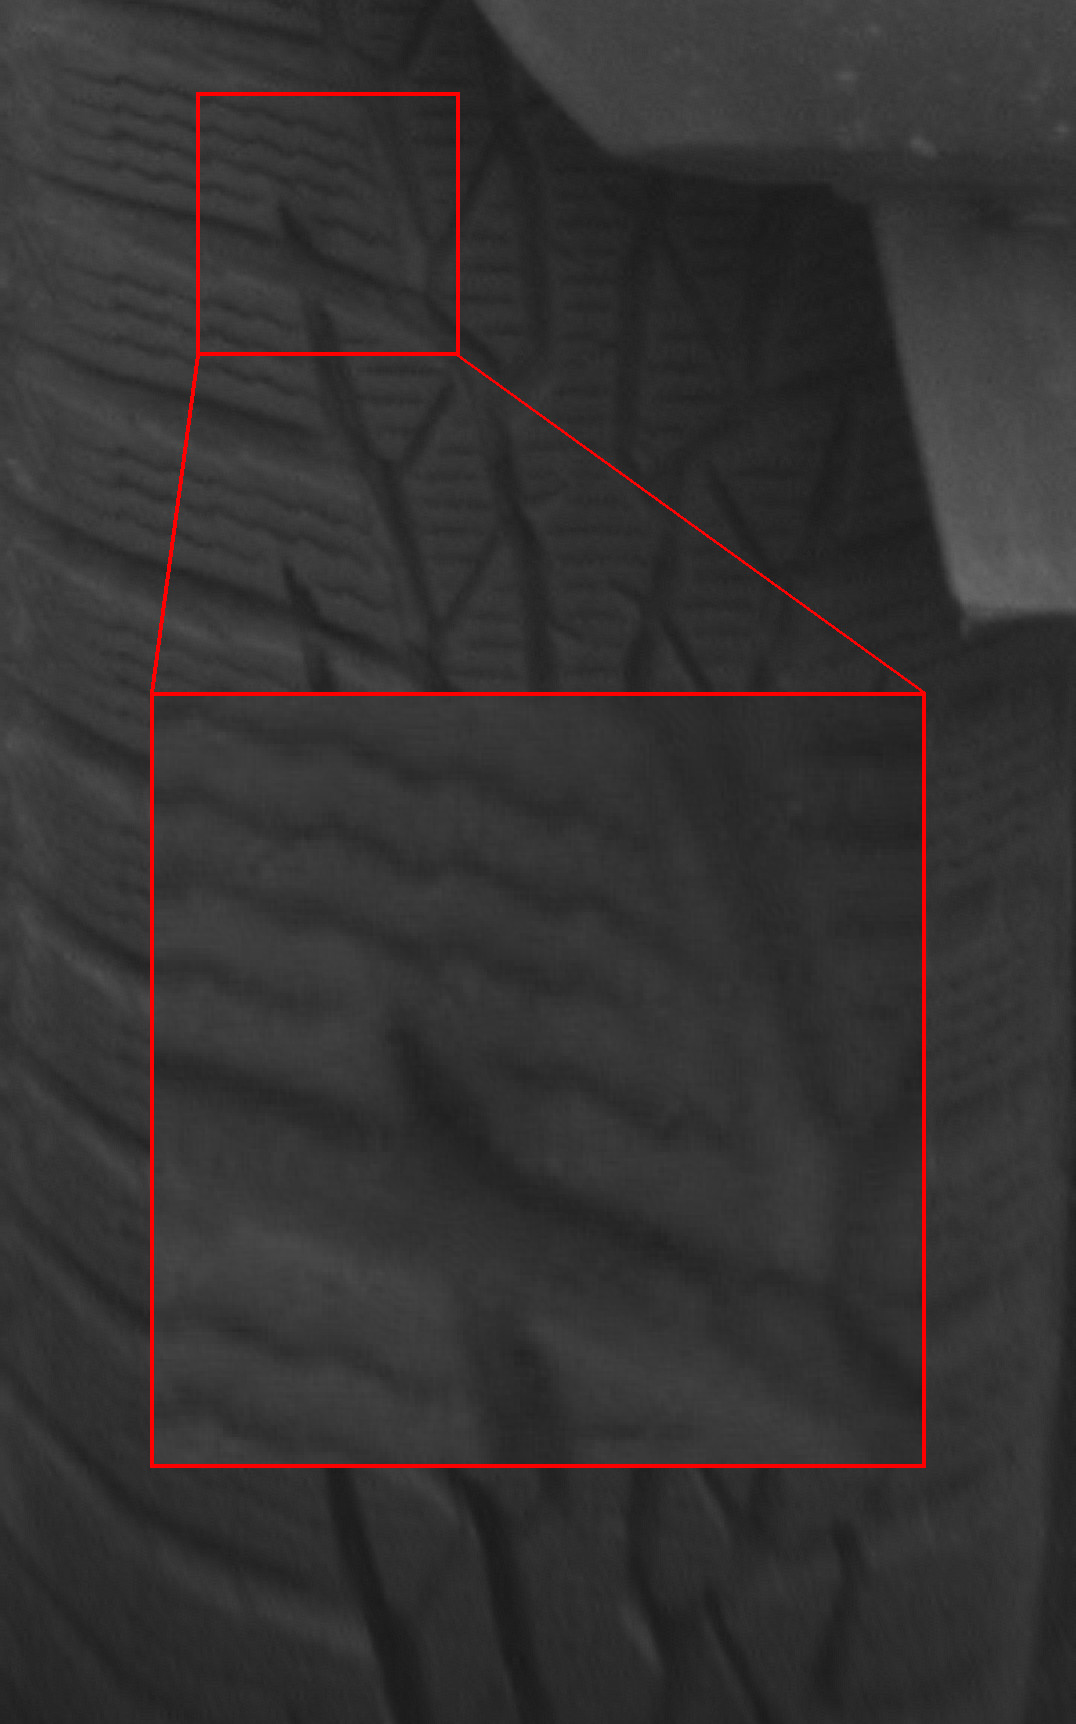
\includegraphics[width=0.2\textwidth]{media/upscaled-250epochs-less-agressive.jpg}
        \label{fig:upscaled-250epochs-less-agressive}
    }
    \subfloat[50 epochs with dropout]{
        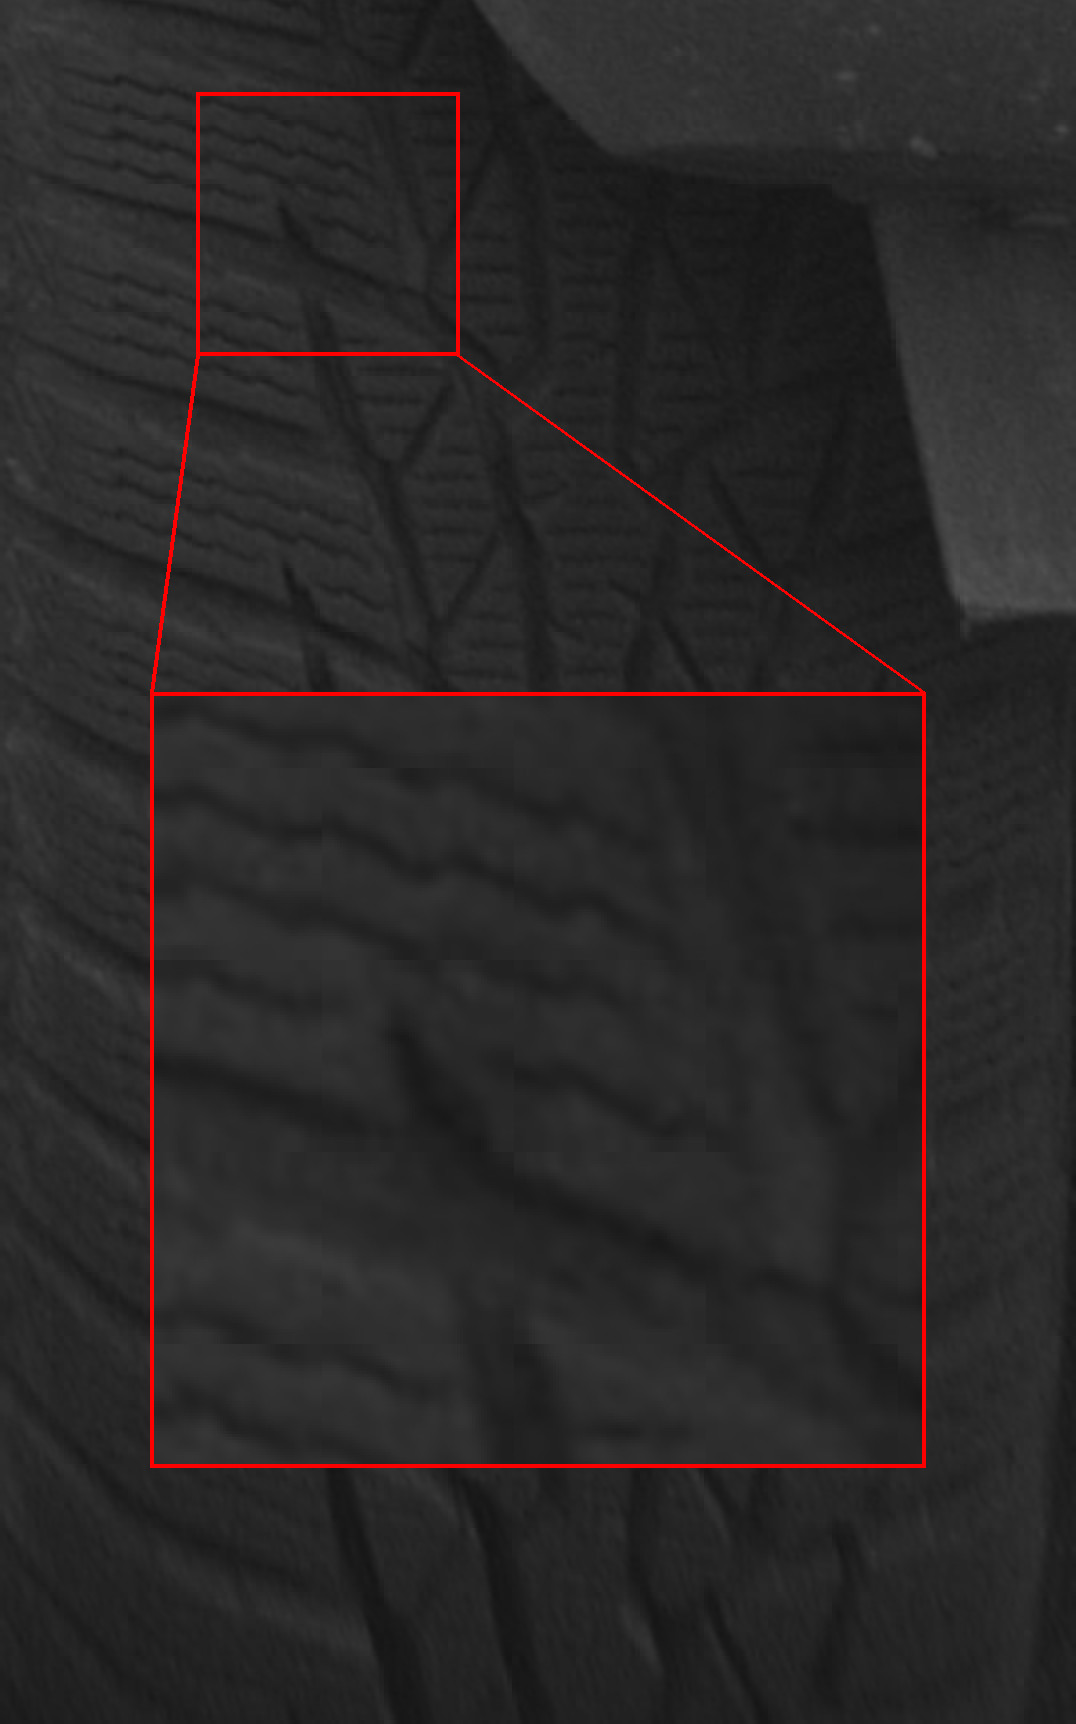
\includegraphics[width=0.2\textwidth]{media/upscaled-dropout.jpg}
        \label{fig:upscaled-dropout}
    }}
    \caption{Examples of upscaled images using trained SRCNN.}
    \label{fig:trained-models}
\end{figure*}

\newpage
\noindent
After just ten epochs, the upscaled images show promising detail. Going further to 250 epochs changes very little, but it does smooth out the rough edges caused by reconstructing the image from $64\times64$ patches. Fig. \ref{fig:trained-models} shows this. It also indicates that upscaling introduces noise in the image. The amount of noise depends on the training data. When the downsampling of training images is toned down, the resulting model does not sharpen the image as much, but it also does not add so much noise, as seen in Fig. \ref{fig:upscaled-250epochs-less-agressive}. Another attempt to reduce noise was made by adding a dropout layer. Dropout works differently in convolutional layers than in fully connected layers \cite{Reinhold2019}. While there is less noise in the upscaled image, it is also darker, as seen in Fig. \ref{fig:upscaled-dropout}.

\begin{figure}[htpb]
  \centering
  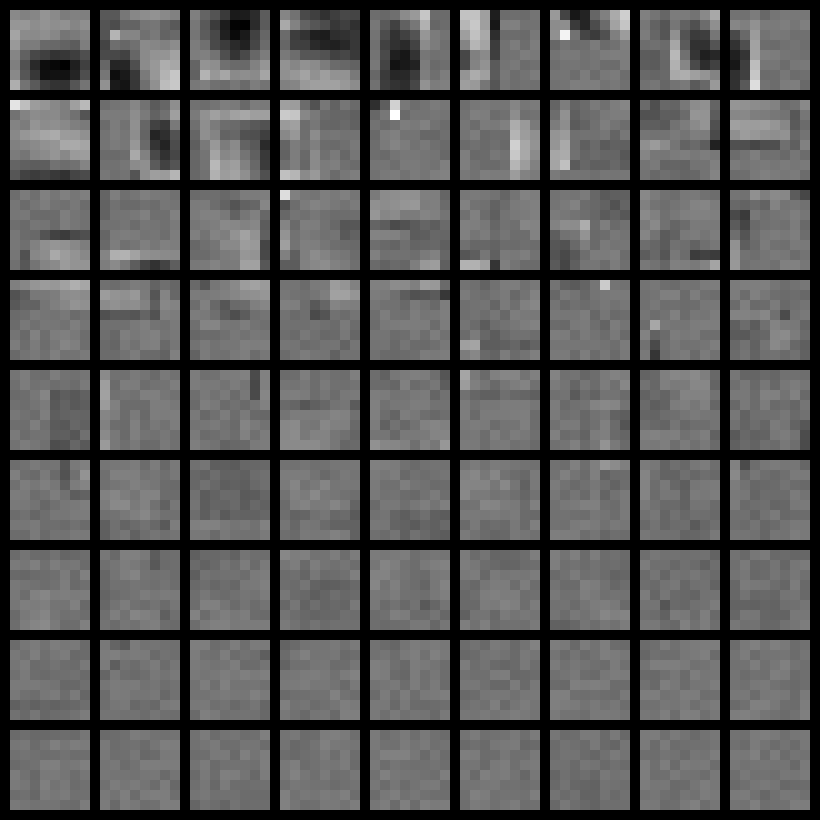
\includegraphics[width=0.95\linewidth]{media/250epochs-learned-filters.png}
  \caption{Learned filters of the first layer.}
  \label{fig:learned-filters}
\end{figure}

Fig. \ref{fig:learned-filters} contains learned filters of the first convolutional layer, sorted by their variance. Many of them seem to not be doing much. This aligns with a similar figure in the original SRCNN paper.

Next, the accuracy of the trained SRCNN will be compared to pretrained  superresolution models implemented in OpenCV \cite{OpenCV}:
\begin{itemize}
  \item EDSR \cite{Lim2017},
  \item ESPCN \cite{Shi2016},
  \item FSRCNN \cite{Dong2016},
  \item LapSRN \cite{Lai2017}.
\end{itemize}

\begin{figure}[htpb]
  \centering
  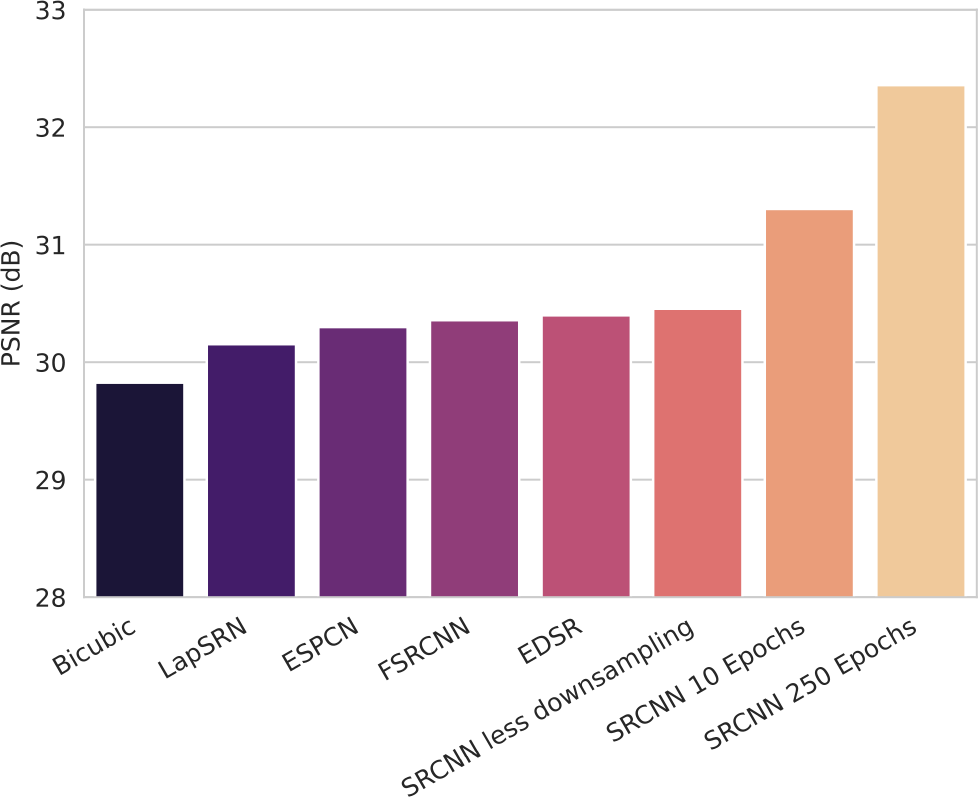
\includegraphics[width=\linewidth]{media/PSNR-comparison.png}
  \caption{PSNR comparison of different models.}
  \label{fig:psnr-comparison}
\end{figure}

Fig. \ref{fig:psnr-comparison} shows the accuracy of different models on the testing images. The dropout model is not included in this figure, as it scored only 18.6 dB.

\section{Conclusion}

While the trained SRCNN is not perfect, as it does introduce some noise, it still provides better results than other models, which have been trained on a larger and more generalized dataset. Unfortunately, training more epochs to see if the noise would be reduced is not feasible on the available hardware (single laptop GPU). Online training services do exist but are either monetized or even slower at training than the RTX 3060 Mobile.

An image can be fed through the SRCNN multiple times (shown in Fig. \ref{fig:multi-example}). However, this further amplifies the added noise, as one would expect.

\begin{figure}[htpb]
    \centerline{
    \subfloat[Original]{
        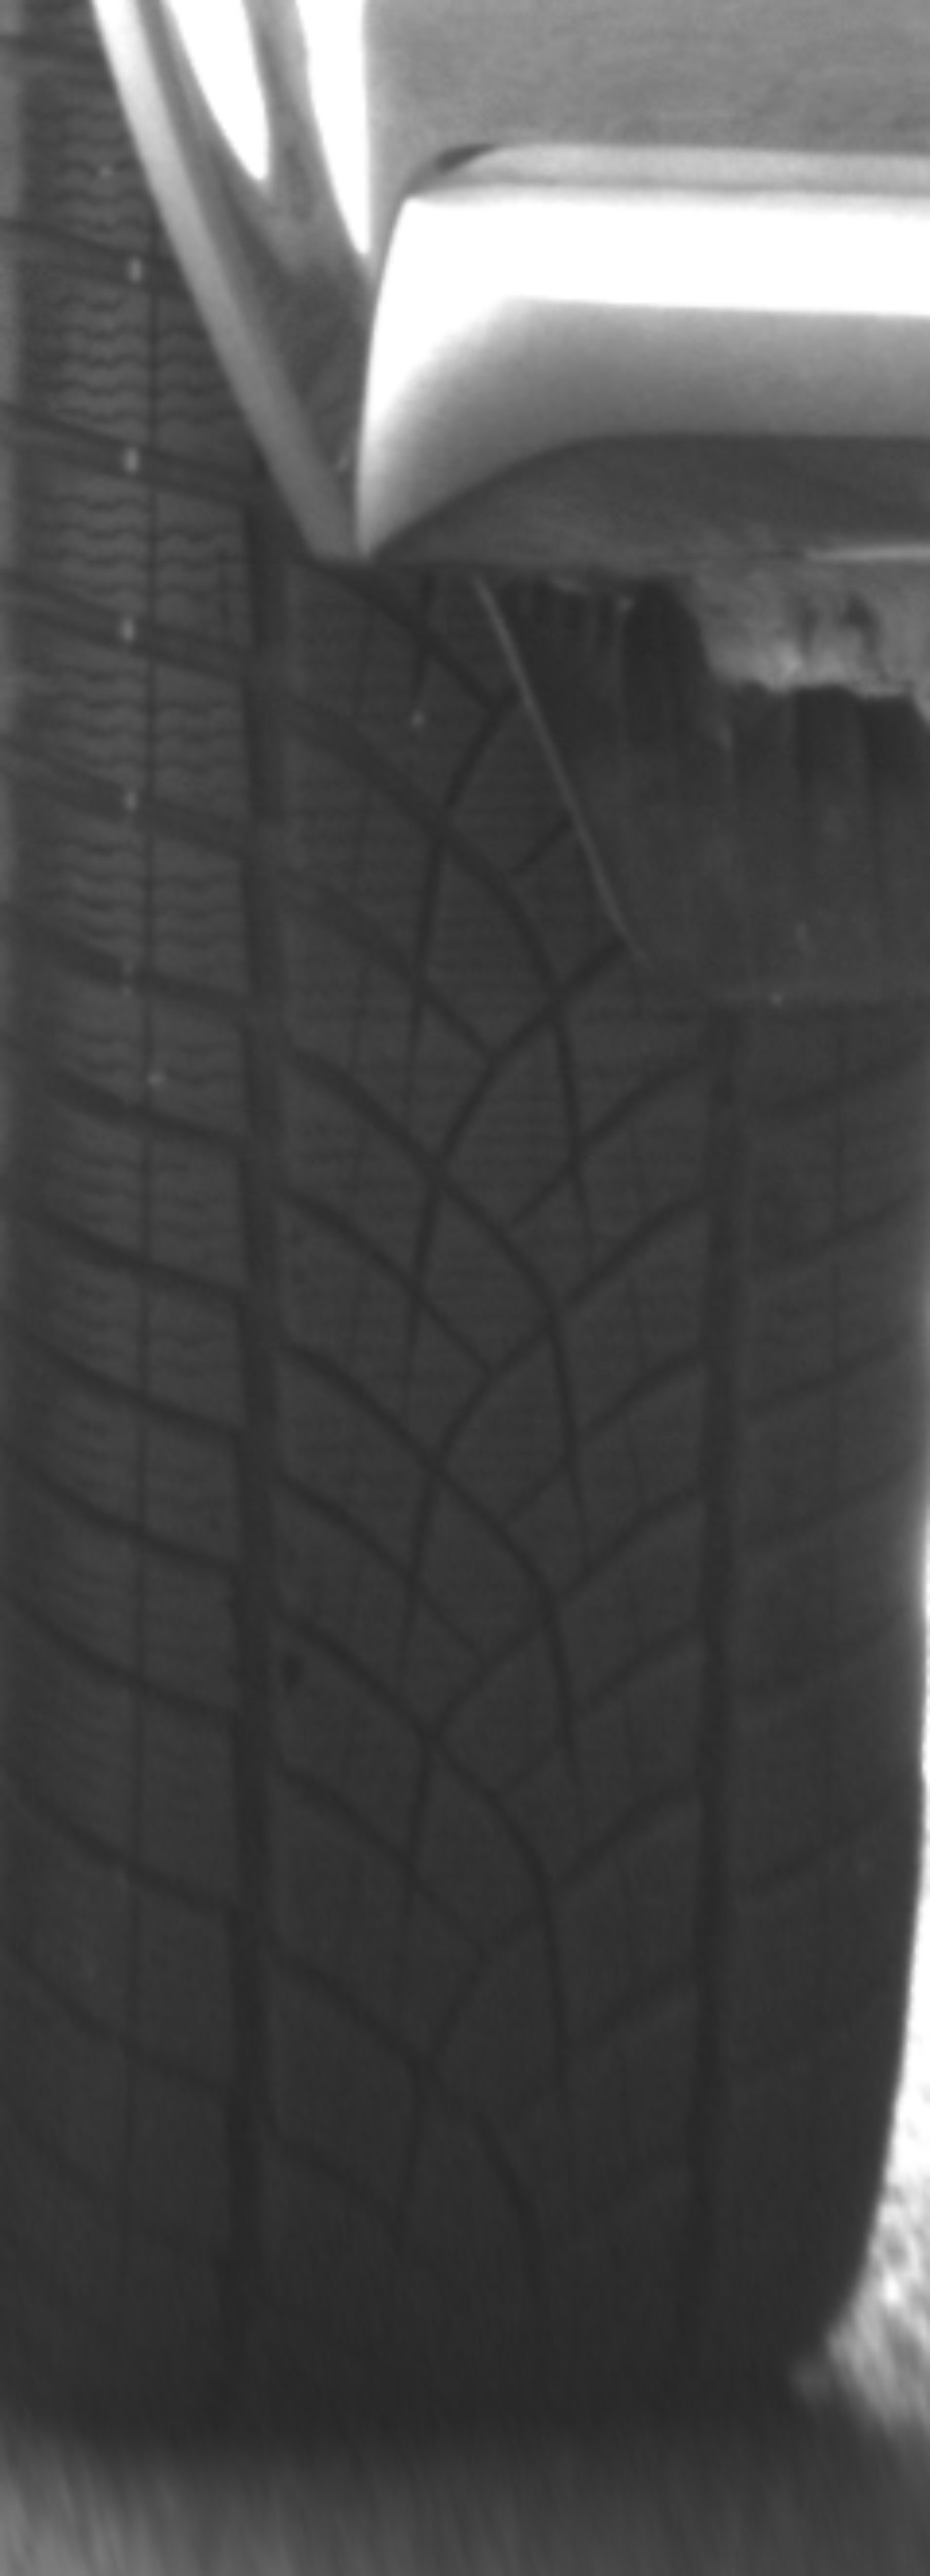
\includegraphics[width=0.15\textwidth]{media/multi-original.jpg}
        \label{fig:multi-original}
    }
    \subfloat[4-times]{
        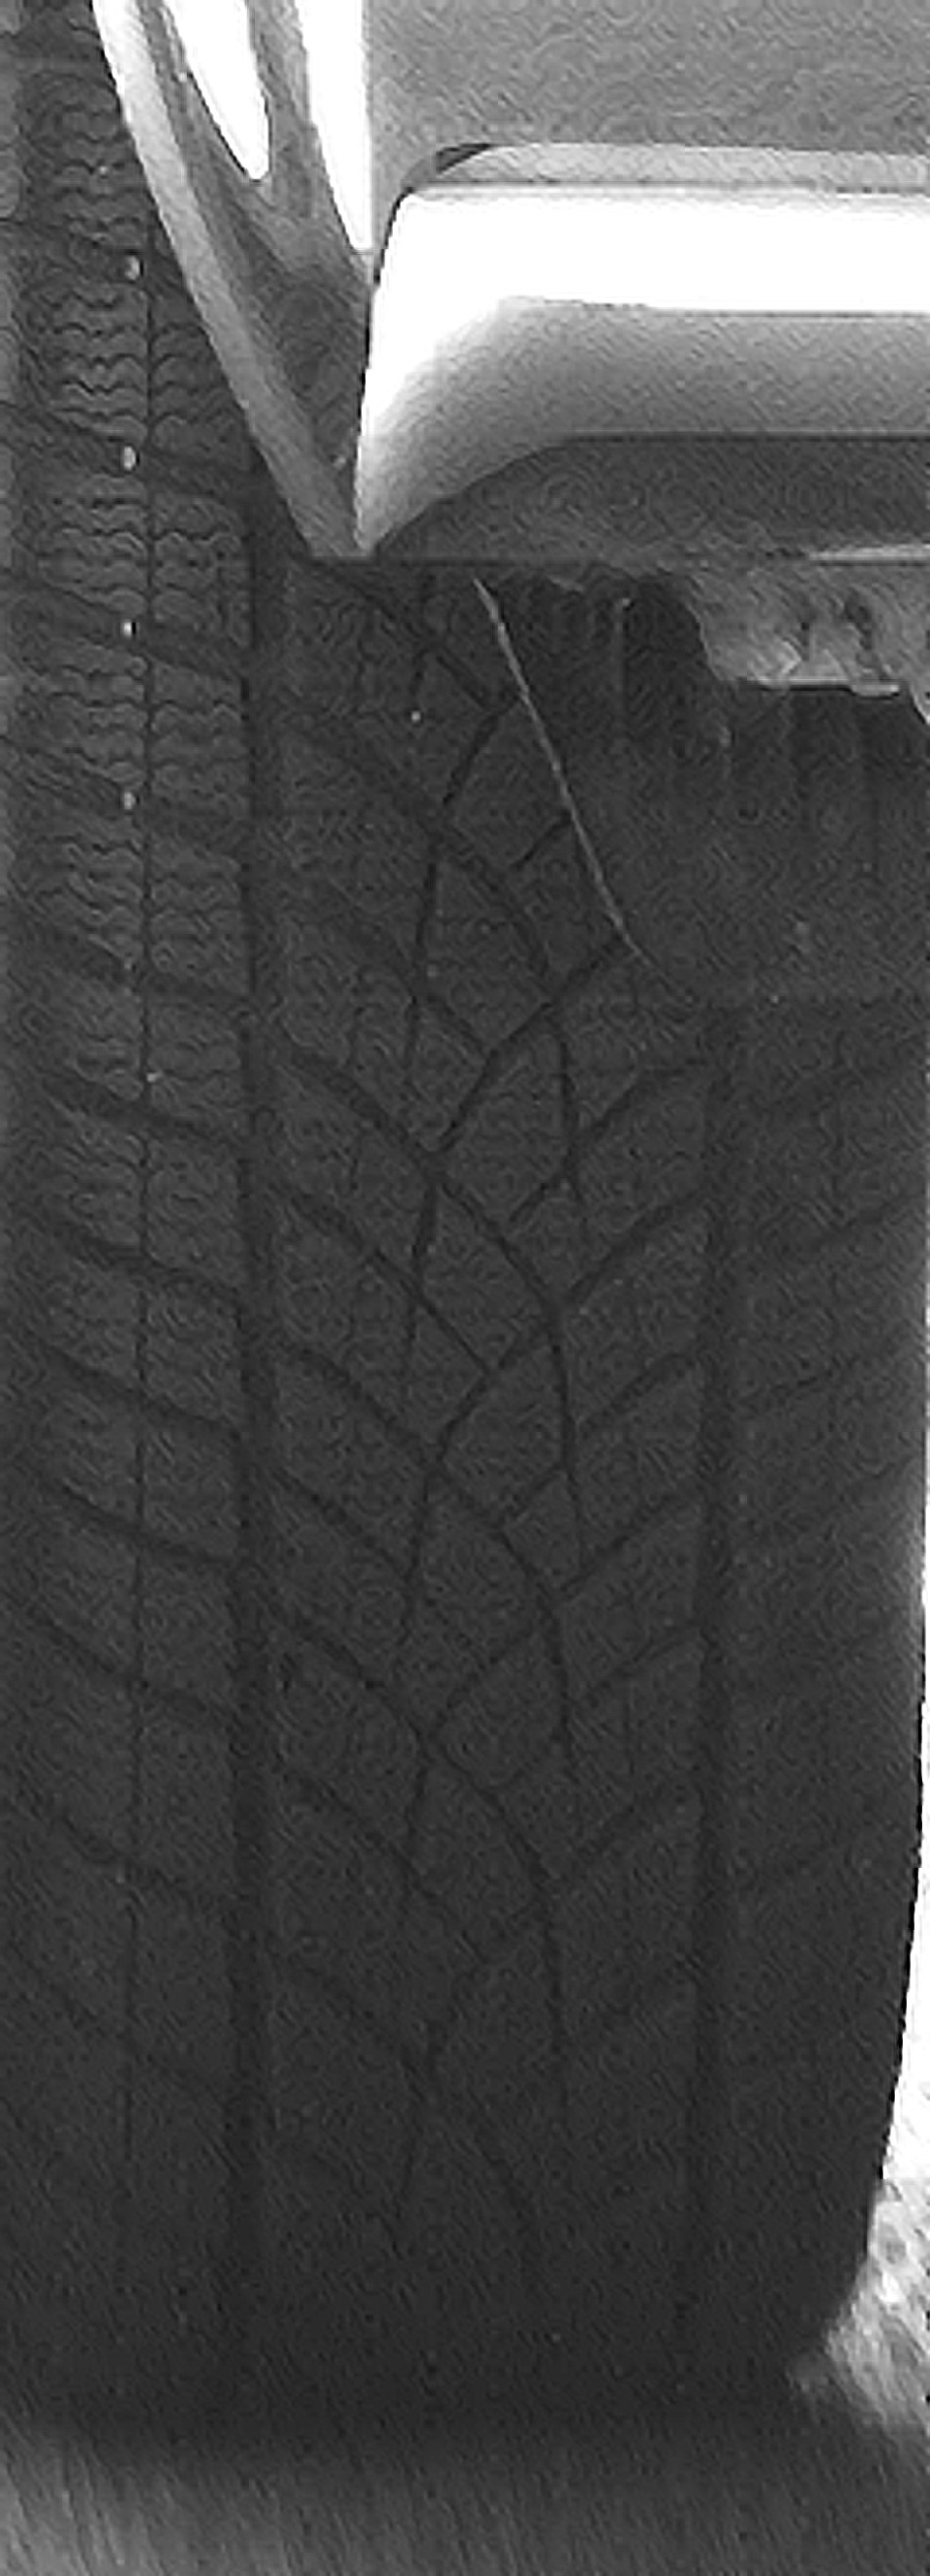
\includegraphics[width=0.15\textwidth]{media/multi-4.jpg}
        \label{fig:multi-4}
    }
    \subfloat[8-times]{
        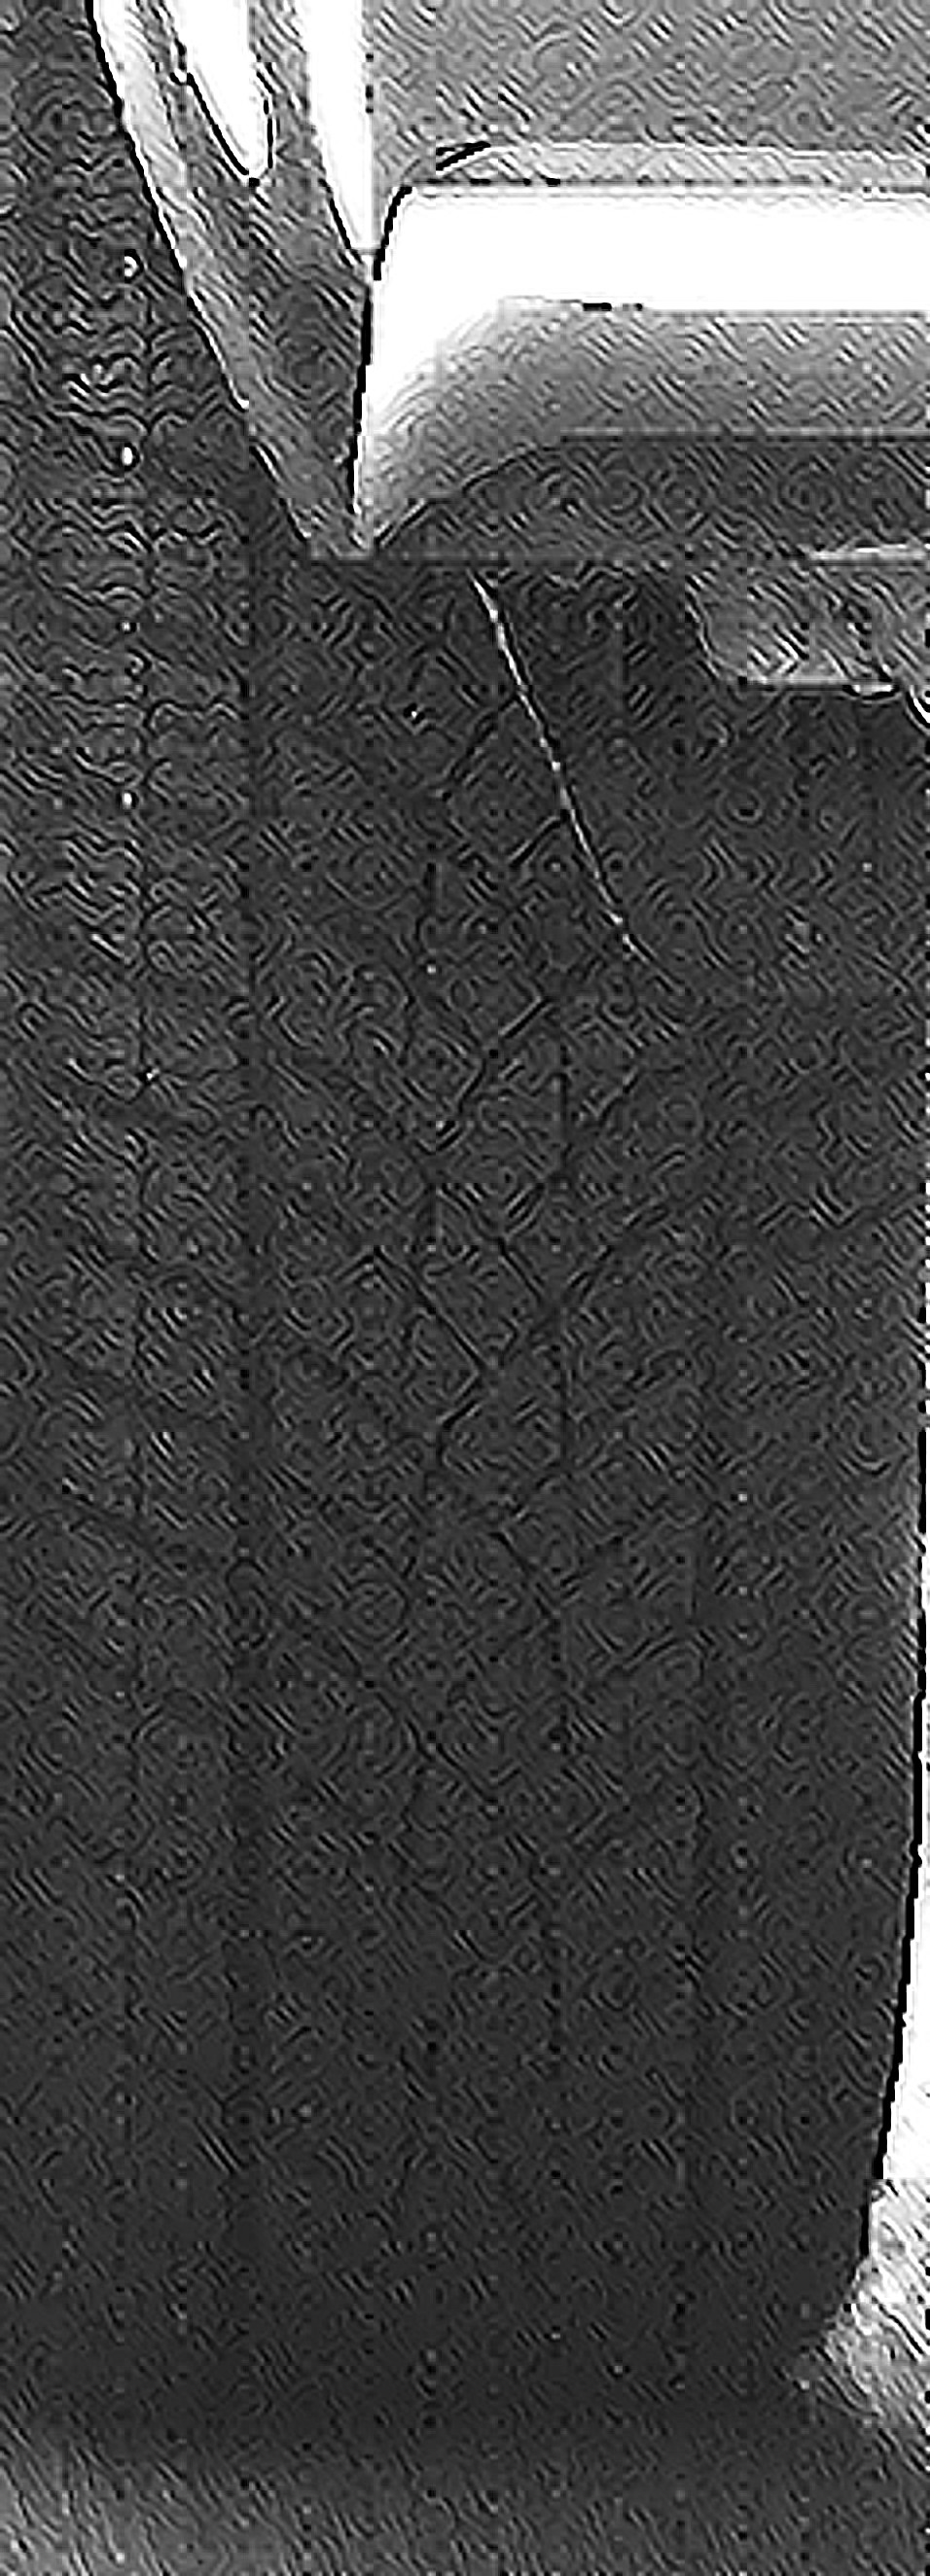
\includegraphics[width=0.15\textwidth]{media/multi-8.jpg}
        \label{fig:multi-8}
    }}
    \caption{Multiple upsamplings.}
    \label{fig:multi-example}
\end{figure}

Apart from more training and better training images (with higher resolution), other superresolution models could be evaluated in the future to determine the best one suited for this very narrow application of upscaling grayscale tire treads.

\begin{thebibliography}{9}
\bibitem{Bohunek2022} D. Bohuněk, ``Návrh kamerového systému pro snímání vzorku pneumatiky'' [Design of a camera system for scanning a tire tread], \textit{Bachelor thesis, FIT CTU}, May. 2022, Available: \url{https://hdl.handle.net/10467/101628}.
\bibitem{Dong2014} C. Dong, C. C. Loy, K. He and X. Tang, ``Image Super-Resolution Using Deep Convolutional Networks,'' \textit{Computer Vision and Pattern Recognition (cs.CV)}, Dec. 2014, doi: \href{https://doi.org/10.48550/arXiv.1501.00092}{10.48550/arXiv.1501.00092}.
\bibitem{Reinhold2019} J. Reinhold, ``Dropout on convolutional layers is weird'', \textit{Towards Data Science}, Feb. 2019, Available: \url{https://towardsdatascience.com/dropout-on-convolutional-layers-is-weird-5c6ab14f19b2}.
\bibitem{OpenCV} OpenCV (Open Source Computer Vision Library) \url{https://opencv.org/}.
\bibitem{Lim2017} B. Lim et al., ``Enhanced Deep Residual Networks for Single Image Super-Resolution'', \textit{Computer Vision and Pattern Recognition (cs.CV)}, Jul. 2017, doi: \href{https://doi.org/10.48550/arXiv.1707.02921}{10.48550/arXiv.1707.02921}.
\bibitem{Shi2016} W. Shi et al., ``Real-Time Single Image and Video Super-Resolution Using an Efficient Sub-Pixel Convolutional Neural Network'', \textit{Computer Vision and Pattern Recognition (cs.CV)}, Sep. 2016, doi: \href{https://doi.org/10.48550/arXiv.1609.05158}{10.48550/arXiv.1609.05158}.
\bibitem{Dong2016} C. Dong, C. C. Loy, X. Tang, ``Accelerating the Super-Resolution Convolutional Neural Network'', \textit{Computer Vision and Pattern Recognition (cs.CV)}, Aug. 2016, doi: \href{https://doi.org/10.48550/arXiv.1608.00367}{10.48550/arXiv.1608.00367}.
\bibitem{Lai2017} W. Lai, J. Huang, N. Ahuja and M. Yang, ``Fast and Accurate Image Super-Resolution with Deep Laplacian Pyramid Networks'', \textit{Computer Vision and Pattern Recognition (cs.CV)}, Oct. 2017, doi: \href{https://doi.org/10.48550/arXiv.1710.01992}{10.48550/arXiv.1710.01992}.
\end{thebibliography}

\end{document}
